\chapter{Viewing Diffraction Data}\label{viewing_data}

Figure~\ref{calibration_tab} shows the 
Area Diffraction Machine's \gui{Calibration} tab. 
The \gui{Data File:} input can be 
used to load diffraction data either by typing in the filename 
and pushing the load button or by clicking on the folder icon and
using the file selector. After the file is loaded, 
the window shown in figure~\ref{diffraction_data_window}.
will open with the diffraction data in it. 

\begin{SCfigure}[1][bthp]
    \centering
    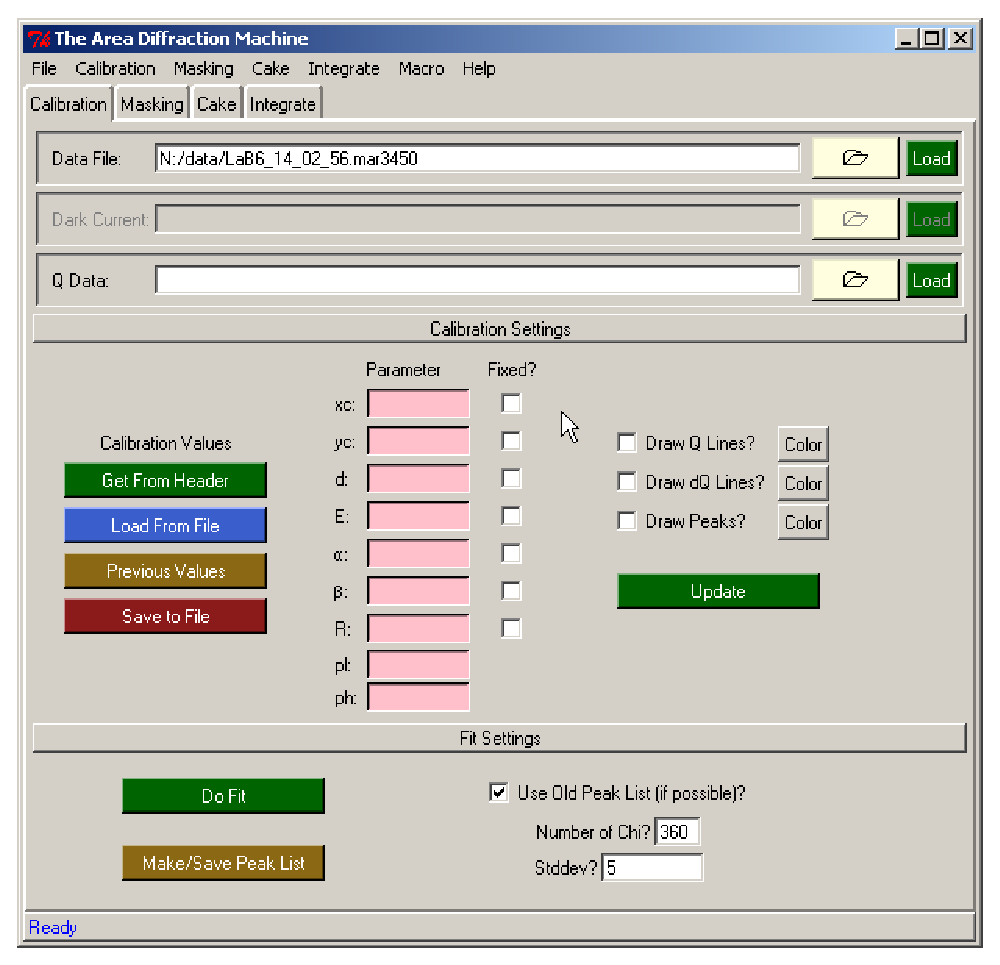
\includegraphics[scale=.75]
    {figures/calibration_tab.eps}
    \caption{The \gui{Calibration} tab. This tab can be used
    to load diffraction data into the program.} 
    \label{calibration_tab}
\end{SCfigure}

\begin{SCfigure}[1][bthp]
    \centering
    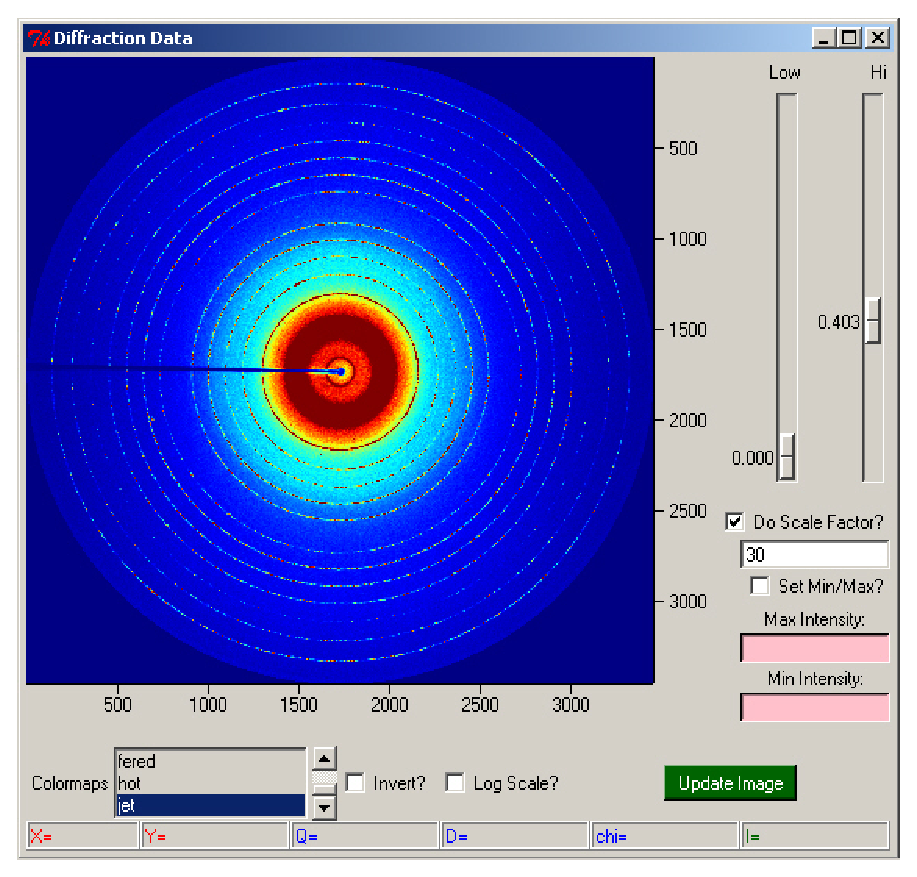
\includegraphics[scale=.75]
    {figures/diffraction_data_window.eps}
    \caption{This diffraction data window will open after 
    a file is loaded.} 
    \label{diffraction_data_window}
\end{SCfigure}

The diffraction data window can be used to interact with 
diffraction data. The window can be used to:
\begin{itemize}
    \item {\em Zoom into the data} -- left click on the data and 
    hold down on the mouse. When moving the mouse around, the
    program will create a resizable square. When the mouse is released,
    the program will zoom into the selected region.
    \item {\em Zoom out of the data} -- right click on
    the data.
    \item {\em Pan across the data} -- hold shift, push down either mouse
    button, and then move the mouse. The image will move 
    with it. Let go of the mouse to stop panning.
    \item {\em Resize the window} -- click on the bottom right corner of
    the window and drag. The window will resize just like any
    other window and the image will become larger or smaller.  
    \item {\em Read coordinates for a selected point} -- when mousing
    over the image, the $x$, $y$, $Q$, $\chi$, and intensity
    values for the current pixel will be displayed at the bottom of the
    window. $Q$ and $\chi$ will only be displayed if valid calibration
    data is loaded into the program. See chapter~\ref{calibration} for
    a discussion of calibration.
    \item {\em Change the Color Map} -- the \gui{Colormaps} selector 
    can be used to change the particular color map used to display the 
    data.
    \item {\em Invert the Color Map} -- The \gui{Invert?} check box can 
    can be used to invert the colors of the color map.
    \item {\em Low \& Hi Pixels} -- The sliders to the right of the 
    image can be used to change the intensity scale of the
    image. The low value corresponds to the percentage of
    the most intensity pixel value that is mapped to the lowest part of
    the color map and the hi value corresponds to the percentage of
    the most intense pixel value that is mapped to the highest 
    part of the color map.  This feature is can make more
    visible certain intensity ranges in the image.
    \item {\em Log Scaling} - By default, intensity values are linearly 
    mapped to colors in the color map. The \gui{Log Scale?} check box 
    can be used to instead apply a log scale mapping of the intensity 
    values to the color map.
\end{itemize}

\section{File Formats}

The program can load the Mar data \macroline{.mar2300}, 
\macroline{.mar3450}, and the \macroline{.mccd} Mar CCD format
It can load standard \macroline{.tiff} data. 
and the ESRF Data Format \macroline{.edf}.
The program can only deal with square data so whenever non-square
data is loaded, the data will be padded out with blank values
until the data is square.

\section{Loading Multiple Images}

The \gui{Data File:} input can be used to load multiple files
at the same time.
If multiple files are typed into the \gui{Data File:} input and
are separated by spaces, they will all be loaded in. 
Alternately, the diffraction data file 
selector can be used to select and load multiple files.
The program will add the intensities of the images pixel by pixel 
and work with the combined image. The program can only add files 
of the same format.

\section{Saving Diffraction Data}
\index{Save}\index{ESRF Data Format}

Diffraction data can be saved as several popular image formats. 
The data can be saved from the \gui{File} menu using 
the \gui{Save Image} option. The formats currently allowed are \gui{jpg}, 
\gui{gif}, \gui{eps}, \gui{pdf}, \gui{bmp}, \gui{png}, \gui{tiff}, and 
the ESRF data format \gui{edf}.

Images saved as a popular image format will contain whatever
threshold masks, polygon masks, $Q$ lines, $\Delta Q$ lines, and peaks 
are currently displayed and they will be saved
at whatever the current zoom level is.\footnote{This is not the case with 
ESRF data. ESRF data will be saved unzoomed with none
of the lines or masks on top of it.} See chapter~\ref{calibration} for 
a discussion of the $Q$ lines, $\Delta Q$ lines, and peaks. See 
chapter~\ref{pixel_masking} for a discussion of threshold masks and 
polygon masks.

Because the program will pad any non-square data when
it is loaded, the program will always save square
images. If this is undesirable, the saved images
will need to be cropped using another program.

